\documentclass[12pt]{article}

\usepackage{ctex}
\usepackage{geometry}
\usepackage{enumerate}
\usepackage{amsmath}
\usepackage{float}
\usepackage{subfigure} 
\usepackage{listings}
\usepackage{xcolor}
\usepackage{cases}
\usepackage{amssymb}    %triangleeq
\usepackage{lastpage}   %页码
\usepackage{fancyhdr}   %页眉页脚
\usepackage{graphicx}   %图片引用路径
\usepackage{indentfirst}    %缩进设置
\usepackage{booktabs}
\usepackage{multirow}

\setlength{\parindent}{2em}%缩进设置
% \graphicspath{{C:/Users/adm/Desktop/课程文件/科学计算/作业/3.9作业/tex/image}}%图片引用Path,好像并没有什么用

%New colors defined below
\definecolor{codegreen}{rgb}{0,0.6,0}
\definecolor{codegray}{rgb}{0.5,0.5,0.5}
\definecolor{codepurple}{rgb}{0.58,0,0.82}
\definecolor{backcolour}{rgb}{0.95,0.95,0.92}

%Code listing style named "mystyle"
\lstdefinestyle{mystyle}{
  backgroundcolor=\color{backcolour},   
  commentstyle=\color{codegreen},
  keywordstyle=\color{magenta},
  numberstyle=\tiny\color{codegray},
  stringstyle=\color{codepurple},
  % basicstyle=\ttfamily\footnotesize,
  basicstyle=\footnotesize,
  breakatwhitespace=false,         
  breaklines=true,                 
  captionpos=b,                    
  keepspaces=true,                 
  numbers=left,                    
  numbersep=5pt,                  
  showspaces=false,                
  showstringspaces=false,
  showtabs=false,                  
  tabsize=2
}

\lstdefinestyle{myPython}{% myPython是格式的名字
	frame=l,
	language=Python,
	aboveskip=3mm,
	belowskip=3mm,
	showstringspaces=false,
	columns=flexible,
	numberstyle=\small\color{red},
	basicstyle={\small\ttfamily},
	keywordstyle=\color{blue},
	commentstyle=\color{codegreen},
	stringstyle=\color{codepurple},
	breaklines=true,
	breakatwhitespace=true,
	tabsize=3
}

%"mystyle" code listing set
\lstset{style=mystyle}

\usepackage{indentfirst}
\setlength{\parindent}{2em}%缩进设置

\graphicspath{{images/}}%图片引用Path
\geometry{left=1in,right=0.75in,top=1in,bottom=1in}     %页边距


\lhead{} %左上页眉

\begin{document}
\pagestyle{fancy}
\setcounter{page}{1}
\rhead{Page \thepage\ of \pageref{LastPage}}
%页码设置
\vspace{20pt}
\centerline{{\Large \textbf{计算机模拟 project1}}}
\vspace{15pt}

\centerline{{\large \textbf{汪奕晨 3180105843}}}
\vspace{10pt}

\centerline{{\large \textbf{数学科学学院\hspace{5pt}数学与应用数学专业}}}
\vspace{15pt}

%============================== Q1 =========================================
%============================= Problem Restatement =============================
\section{问题描述}
\begin{enumerate}
    \item 用简单遗传算法求解TSP问题
    \item 比较简单遗传算法与模拟退火算法在各方面的优劣
    \item 提高遗传算法的收敛性与收敛率,并验证想法
    \item 结合遗传算法和模拟退火算法构建出更加先进的算法
\end{enumerate}

% 具体要求:
% \begin{enumerate}
%     \item 城市的产生参照第五章的做法随机产生
%     \item 交叉变异算子和DNA编码可以采用笔记的方式,也可以自己设计
%     \item 代码可以采用Matlab或Python,但项目报告必须以pdf的形式提交,代码作为附件上传并不计入篇幅
%     \item 键入问题和算法思路,对于新引入的内容如果没有代码分析也可以用是党的理论分析代替
%     \item 请在20-200的规模内测试你的算法,结果以图标的形式包含在报告里并做简要的分析
%     \item 在最后用一段话对你的报告做出总结
%     \item 鼓励查阅文献和讨论,但每一份报告必须独立完成,报告最后附加参考文献,并在适当位置标出引用
%     \item 本次报告正文连同图表,公式,不得超过10页。
% \end{enumerate}

%=================================== Notations ===========================
\section{Notations}
\begin{table}[H]
  \centering
  \begin{tabular}{cc}
    \hline
    记号 & 含义 \\ \hline
    $N$ & TSP实例中城市的数目 \\
    $G$ &  使用GA算法时种群的大小\\
    $M$ & GA算法中迭代次数,在SA算法中指降温次数\\
    $I$ & SA算法中每个温度的迭代次数\\
    $p_r,p_c,p_m$ & GA算法中生成子代时复制(repeat),交叉(cross),突变(mutate)的概率\\
    \hline
  \end{tabular}
  \caption{Notations}
  \label{tab: Notations}
\end{table}

%============================= Theory and Algorithms =============================
\section{设计思路}
\subsection{简单遗传算法的设计思路}
\subsubsection{适合度计算}
由于TSP算法的目的是要\textbf{最小化}环游距离,而遗传算法中需要\textbf{最大化}适合度,我们使用种群中最大环游距离减去各样本的环游距离作为各样本的适合度。
尽管这会使得不同代数的种群适合度无法比较(因为种群的最大距离也在不断变化),但在算法中并不需要我们比较不属于同一子代个体的适合度,因此该方法不会造成逻辑上的错误。

\subsubsection{遗传计算}
根据$p_r,p_c,p_m$的比例,决定自带的每个个体时进行轮盘赌抽取决定要进行复制、交叉或突变。在具体的实现上,
我们总是先通过抽取得到子代分别由复制、交叉、突变而来的个体数目,而后再批量生成各遗传方式得到的子代。

\textbf{选择算子:}

在最初的尝试中,我们直接使用轮盘赌抽取实现选择算子,但这并不能导致最短距离随着迭代次数收敛。

于是我们优化为采用2-锦标赛进行选择复制。根据上代各亲本适合度的比例通过随机数抽取$n_r$个子代作为一组,为了保证子代的多样性,同一父本不会被重复抽取。共抽取两组。
选择两组中对应位置表现最好(有更短的距离/更高的适合度)的复制到子代。

相比于轮盘赌抽取,锦标赛抽取可以更好地选出优质的个体,同时也保留了跳出局部最优的机会。在应用中有更好的表现。

\textbf{交叉算子:}

分别实现讲义中'partial-mapped', 'order', 'position-based'三种交叉方法,在之后对各交叉方法的性能进行对比。

\textbf{变异算子:}

随机抽取$n$-排列中的两个位置,对其之间的环游进行反向。

\subsubsection{$p_r,p_c,p_m$比例的自适应修改方法}
一种朴素的想法是,当交叉/突变效果较好时则增大交叉/突变概率。我们采用Equation (\ref{eq: auto p})中的方式自适应调整比例\cite{Ref1}。

\begin{equation}
    \begin{aligned}
        p_c = \left\{
        \begin{array}{cc}
            K_1\frac{F_{max} - F'}{F_{max} - F_{avg}} & F' > F_{avg} \\
            K_2 & F' \le F_{avg}
        \end{array} 
        \right.
        \\
        p_m = \left\{
        \begin{array}{cc}
            K_3\frac{F_{max} - F''}{F_{max} - F_{avg}} & F'' > F_{avg} \\
            K_4 & F'' \le F_{avg}
        \end{array} 
        \right.
    \end{aligned}    
    \label{eq: auto p}
\end{equation}
$F_{max},F_{avg}$为种群中适应度的最大值与平均值,$F',F''$分别为交叉得到子代与突变得到子代的平均适应度,$K_i,i=1,2,3,4$为超参数,本文中设定为$ (0.5, 0.3, 0.25, 0.15)$。

\subsection{代码设计思路}
这里给出一些实现难点的伪代码以及实现中采用的技巧。对三种交叉算法我们仅介绍最复杂的partial mapped方法,剩余两个方法可以通过np.in1d方法快速实现,具体参考附录中的代码。
\begin{lstlisting}[language = Python, caption = partial-mapped 方法实现交叉]
  def cross_partial_mapped(path_1, path_2, node_1, node_2):
    '''
    输入:path_1,path_2 分别为两个不同的 n - 排列,node_1,node_2 为交换的节点位置
    输出:path_1,path_2 为可变对象, 更改path_1 为交叉后的值
    '''
    cross_part = path_2 中需要交叉到path_1 的点集
    for 遍历path_1 中的每个位置:
      if 该位置不在cross_part 中:
        x = 该位置上的值 
        while 当x 在cross_part 中时:
          找到path_2 中对应位置对应的path_1 中的值 y
          x = y

    将path_1 中需要交换的位置赋值为cross_part
\end{lstlisting}

% 由于我们将GA算法封装为一个类,这里仅介绍需要记录的实例属性与核心迭代的代码设计思路
% \begin{lstlisting}[language = python, caption = GA算法伪代码]
%   class TSP_GA():
%     def __init__(self, inputs):
%       # 需要记录的值有
%       self.dots # 2*n 的点列数据
%       self.n # TSP 规模,即点的多少
%       self.graph # 为n*n 的矩阵,记录点i 到点j 的距离,防止重复计算
%       self.p # pr,pc,pr
%       self.k # 自适应方法中用到的k
%       self.min_record # 记录迭代过程中每一代的最小距离
%       self.mean_record # 记录迭代过程中每一代的平均距离
%       self.best_ans  # 记录整个过程中的最优解
%       self.min_dist # 记录整个过程中最短距离

%       self.group # 种群记录,初始化时随机生成 这里可以调用np.shuffle 方法实现
%       self.distance # 种群中每个个体对应的TSP 距离
%       self.fitness # 种群中每个个体的适合度

%     def reproduce(self, method, auto):
%       '''
%       用于迭代一次的方法,
%       inputs: method 输入说明选择的交叉方法,auto=True 表明是否需要自适应修改self.p
%       '''
%       基于self.fitness 进行一次轮盘赌抽取得到nr,nc,nm,分别为进行选择,交叉,突变的个体数目 
%       # 调用np.choice 可以快速实现

%       通过调用2-锦标赛选择算法抽取nr 个个体遗传到子代
%       通过调用method 对应的交叉方法得到nc 个个体遗传到子代
%       通过轮盘赌抽取nm 个个体,分别进行突变后遗传到子代

%       得到下一代种群next_group,并相应计算next_distance, next_fitness
%       if auto is True:
%         根据以上结果,自适应地更新self.p 即pr,pc,pm
%       更新self.group, self.distance, self.fitness
    

%     def evolute(self,gennerations, method, auto):
%       '''
%       主体迭代方法
%       inputs: gennerations:迭代次数, method:交叉方法, auto:是否采用自适应修改self.p
%       '''
%       根据Generations 生成初始的min_record, mean_record 向量
%       # 用于记录迭代中每代的最小距离与最优距离
%       # 这里是记录整体迭代中的最优解,若先前已有记录则复用先前的,没有则采用65535作为最大值
%       for i in range(gennerations):
%         self.reproduce(method=method, auto=auto) # 调用reproduce 方法迭代一次
%         if 当前种群最小距离 < self.min_dist:
%           更新self.min_dist
%           更新self.best_ans

%         计算当前最短距离,平均距离,存入min_record, mean_record 中

%       更新self.min_record, self.mean_record # 使用np.append 可以在向量后添加新的向量

% \end{lstlisting}

%============================= Results =============================
\section{模拟结果与分析}

\subsection{GA算法的有效性}
对$N=50,G=200,M=300$的参数进行测试,结果如Figure (\ref{pic: Sample})
\begin{figure}[H]
  \centering
  \subfigure[Performance $N=50,G=200,M=300$]{
  \begin{minipage}[t]{0.4\linewidth}
  \centering
  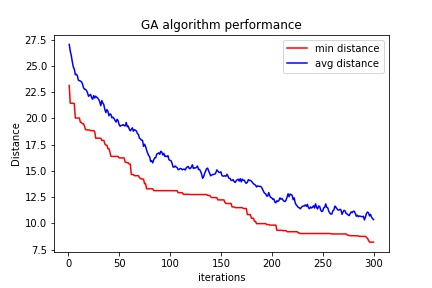
\includegraphics[width=7.5cm]{../figure/GA_perf_50_200_300.jpg}
  \label{pic: Sample perf}
  \end{minipage}
  }
  \subfigure[Result $N=50,G=200,M=300$]{
  \begin{minipage}[t]{0.4\linewidth}
  \centering
  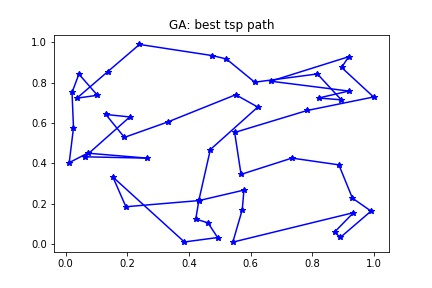
\includegraphics[width=7.5cm]{../figure/GA_res_50_200_300.jpg}
  \label{pic: Sample res}
  \end{minipage}
  }
  \caption{Sample Performance and Result}
  \label{pic: Sample}
\end{figure}

可以看到随着迭代不断进行,最短距离确实在不断地降低,且解也在向最优逼近。
此外,最短距离和种群平均距离以相同的趋势下降,在后文中我们将仅适用最短距离的变化来衡量下降趋势。

\subsection{交叉方法的选择}
分别使用三种交叉策略对不同的参数进行计算,得到的结果如Figure (\ref{pic: cross methods 1},\ref{pic: cross methods 2})
% \begin{figure}[H]
%     \centering
%     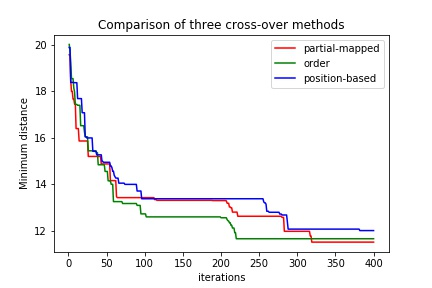
\includegraphics[height = 7cm]{../figure/cross_method_test.jpg}
%     \caption{Result of Three Cross Methods}
%     \label{pic: cross methods test}
% \end{figure}

\begin{figure}[H]
    \centering
    \subfigure[$N=50,G=150,M=750$]{
    \begin{minipage}[t]{0.4\linewidth}
    \centering
    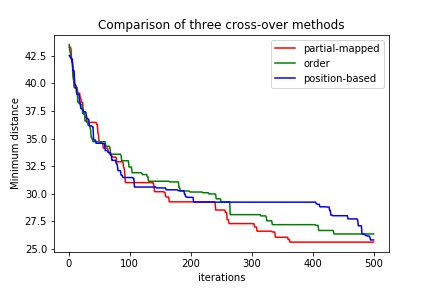
\includegraphics[width=7.5cm]{../figure/cross_method_test_50_150_750_4.jpg}
    \label{pic: cross methods 1}
    \end{minipage}
    }
    \subfigure[$N=25,G=50,M=500$]{
    \begin{minipage}[t]{0.4\linewidth}
    \centering
    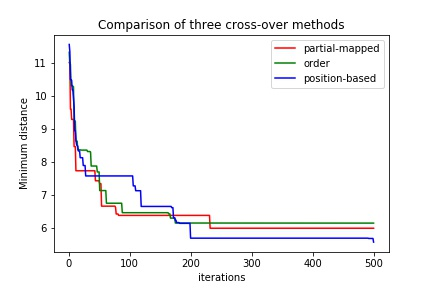
\includegraphics[width=7.5cm]{../figure/cross_method_test_25_50_500_3.jpg}
    \label{pic: cross methods 2}
    \end{minipage}
    }
    \caption{Cross Methods Comparison}
\end{figure}

可以看出在不同的参数下,三种方法最终均会收敛到相近的结果,相对优劣也有偶然因素,我们可以认为三种交叉方法并没有显著的优劣之分。
在后文中我们将默认使用partial-mapped方法。

\subsection{自适应方法的测试}
为了说明自适应方法的有效性,我们选取固定$p_{c,const}=0.4,p_{m,const}=0.2$与$K_1 = 0.5, K_2 = 0.3, K_3 = 0.3, K_4 = 0.15$两组参数进行对比。对比Equation (\ref{eq: auto p}),
目的是让自适应的$p_c$在交叉子代效果较好时会变大,在子代效果不佳时会变小,$(K_1 + K_2)/2 = p_{c,const}$则保证了$p_c$在$p_{c,const}$附近波动,$p_m$同理。
这样在前期种群较为随机时可以加强交叉、变异迅速筛选优势个体,后期种群表现较优异时可以通过降低$p_c,p_m$让解减小波动,迅速收敛。

选取$N=100,G=200,M=1000$分别对同一初始化种群采用自适应与固定值求解,结果如Figure (\ref{pic: GA auto test}).
可以看出自适应的方法确实可以加快GA算法的收敛速度,后文默认采用自适应的方法,$K_i$的取值分别为$(0.5, 0.3, 0.25, 0.15)$

\begin{figure}[H]
  \centering
  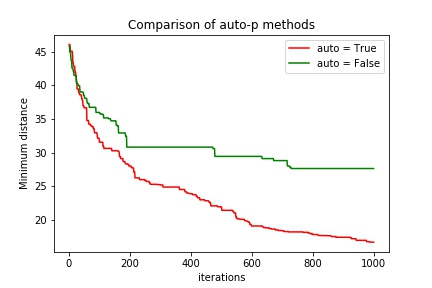
\includegraphics[height = 6cm]{../figure/GA_auto_test_100_200_1000_1.jpg}
  \caption{Automatic $p$ versus Constant $p$}
  \label{pic: GA auto test}
\end{figure}


\subsection{不同规模TSP问题的GA算法求解结果}

\begin{figure}[H]
  \centering
  \subfigure[$N=30,G=100,M=500$]{
  \begin{minipage}[t]{0.4\linewidth}
  \centering
  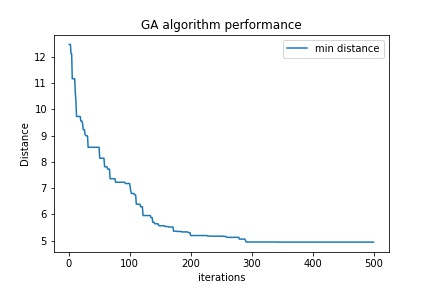
\includegraphics[width=7.5cm]{../figure/GA_perf_30_100_500.jpg}
  \label{pic: GA perf 1}
  \end{minipage}
  }
  \subfigure[$N=30,G=100,M=500$]{
  \begin{minipage}[t]{0.4\linewidth}
  \centering
  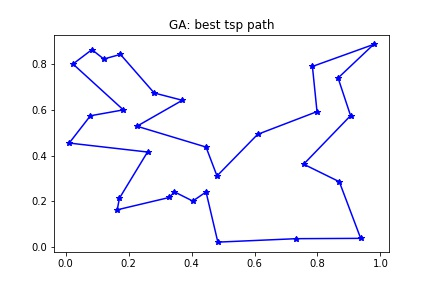
\includegraphics[width=7.5cm]{../figure/GA_res_30_100_500.jpg}
  \label{pic: GA res 1}
  \end{minipage}
  }

  \subfigure[$N=50,G=200,M=1000$]{
  \begin{minipage}[t]{0.4\linewidth}
  \centering
  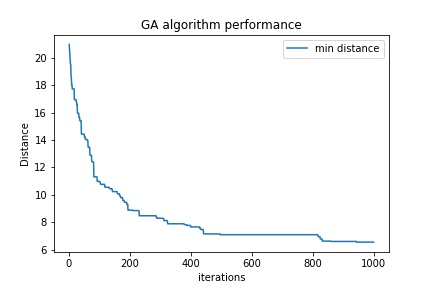
\includegraphics[width=7.5cm]{../figure/GA_perf_50_200_1000.jpg}
  \label{pic: GA perf 2}
  \end{minipage}
  }
  \subfigure[$N=50,G=200,M=1000$]{
  \begin{minipage}[t]{0.4\linewidth}
  \centering
  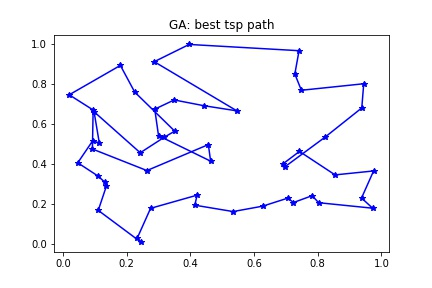
\includegraphics[width=7.5cm]{../figure/GA_res_50_200_1000.jpg}
  \label{pic: GA res 2}
  \end{minipage}
  }
  \caption{GA result for small $N$}
  \label{pic: GA small N}
\end{figure}

如Figure (\ref{pic: GA small N}),当$N$较小时,GA算法可以给出比较好的结果。

如Figure (\ref{pic: GA large N}),当$N$比较大时,GA算法很容易陷入局部最优,给出一个不太好的结果。
且从距离下降的趋势来看,增加迭代次数也并不能使算法更加接近最优解。如对$N=200,G=200$迭代5800次,仍然不能给出一个较好的解

\begin{figure}[H]
  \centering
  \subfigure[$N=100,G=200,M=1000$]{
  \begin{minipage}[t]{0.4\linewidth}
  \centering
  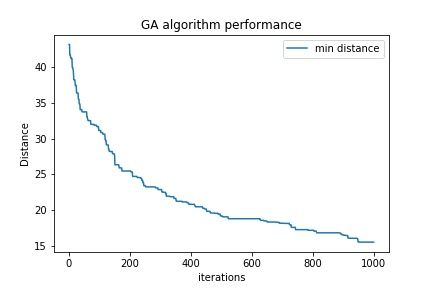
\includegraphics[width=7.5cm]{../figure/GA_perf_100_200_1000.jpg}
  \label{pic: GA perf 3}
  \end{minipage}
  }
  \subfigure[$N=100,G=200,M=1000$]{
  \begin{minipage}[t]{0.4\linewidth}
  \centering
  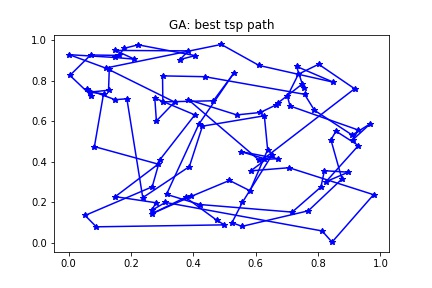
\includegraphics[width=7.5cm]{../figure/GA_res_100_200_1000.jpg}
  \label{pic: GA res 3}
  \end{minipage}
  }

  \subfigure[$N=200,G=200,M=5800$]{
  \begin{minipage}[t]{0.4\linewidth}
  \centering
  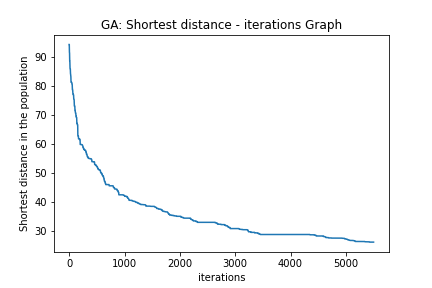
\includegraphics[width=7.5cm]{../figure/GA_perf_200_200_5800.png}
  \label{pic: GA perf 4}
  \end{minipage}
  }
  \subfigure[$N=200,G=200,M=5800$]{
  \begin{minipage}[t]{0.4\linewidth}
  \centering
  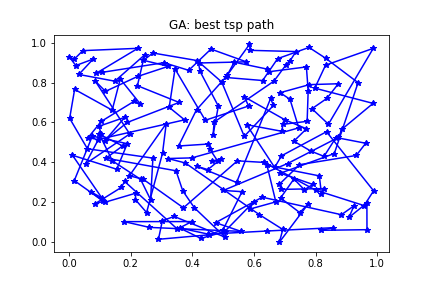
\includegraphics[width=7.5cm]{../figure/GA_res_200_200_5800.png}
  \label{pic: GA res 4}
  \end{minipage}
  }
  \caption{GA result for large $N$}
  \label{pic: GA large N}
\end{figure}



\subsection{GA算法与SA算法的优劣对比}
选取$N=100,G=200,I=600,M=1000$,对较大的参数,可以认为具有一定的普遍性,两种算法运行结果如Figure (\ref{pic: comparison GA SA})
\begin{figure}[H]
    \centering
    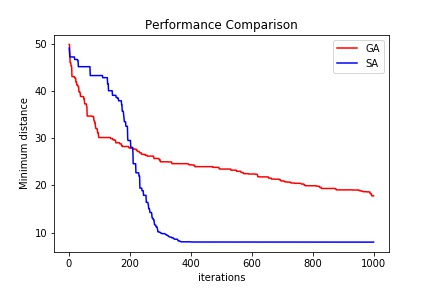
\includegraphics[height = 6cm]{../figure/Compare_GASA_test_100_200_1000_1.jpg}
    \caption{Comparison of GA and SA}
    \label{pic: comparison GA SA}
\end{figure}

可见,在前期GA算法有较快的收敛速度,但当达到足够的迭代次数后,SA算法相比于GA算法会更快地接近最优值。
此外,在本例的参数下,SA算法也比GA算法有更快的运行速度。尽管这可能有代码优化的原因,但我们仍然可以认为SA算法是优于GA算法的。


%==================================== SA in GA ===========================================================
\section{GA算法引入Boltzman生存机制的改进}
\label{sec: SA in GA}

为了改进GA算法的表现,我们尝试在其中融入Boltzman生存机制,即产生交叉、突变的子代时,根据适合度计算$h = \min (1, e^{(new-old)/t})$,其中$new,old$分别为子代与亲代的适合度,$t$为当前温度,每次迭代时按照
$t = t * (1 - 1 / (50 + \ln(iter + 1)))$,$iter$为迭代次数。思想即来源于SA算法。

但仅仅做出以上改变,会使得GA算法中的种群早熟,种群多样性减小,如Figure (\ref{pic: GA SA group variety})
\begin{figure}[H]
  \centering
  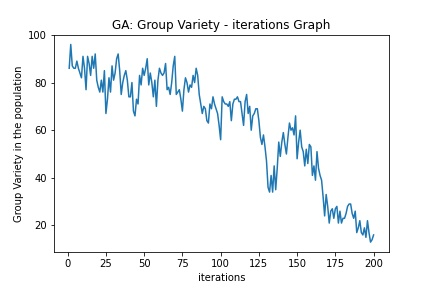
\includegraphics[height = 6cm]{../figure/GA_SA_group_variety.jpg}
  \caption{Group Variety in Improved GA Algorithm}
  \label{pic: GA SA group variety}
\end{figure}

这时需要我们引入防早熟的机制,这里采用最粗暴的方法,每次迭代时剔除种群中的重复个体,使用随机生成的个体去补全使得种群个数保持恒定。
采用这个方法对$N=200,G=200,M=5800$得到的结果如Figure (\ref{pic: GA SA}),对比Figure (\ref{pic: GA res 4}),已经有较好的结果,但相比于SA算法给出的结果,仍然较劣。

\begin{figure}[H]
  \centering
  \subfigure[$N=200,G=200,M=5800$ Improved GA]{
  \begin{minipage}[t]{0.4\linewidth}
  \centering
  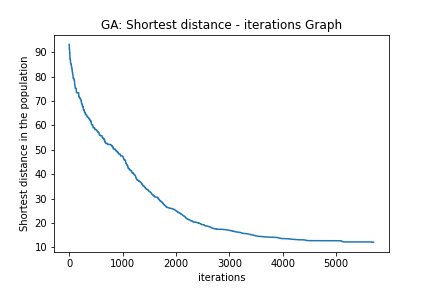
\includegraphics[width=7.5cm]{../figure/GASA_perf_200_200_5800.png}
  \label{pic: GA SA perf}
  \end{minipage}
  }
  \subfigure[$N=200,G=200,M=5800$ Improved GA]{
  \begin{minipage}[t]{0.4\linewidth}
  \centering
  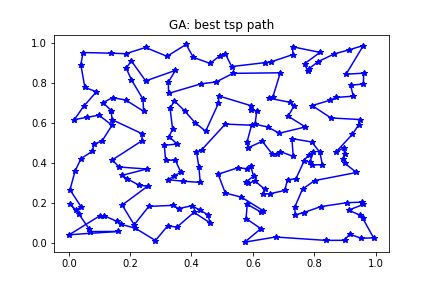
\includegraphics[width=7.5cm]{../figure/GASA_res_200_200_5800.png}
  \label{pic: GA SA res}
  \end{minipage}
  }
  \caption{GA result for large $N$}
  \label{pic: GA SA}
\end{figure}

%============================= Conclution and Disscusion =============================
\section{结论与改进}

\subsection{GA算法的改进}
\begin{enumerate}
    \item 在GA算法迭代过程中,总是执行固定的迭代次数。使得对不同的$N$与$G$需要人工调整$M$以得到更好的解。如果设定提前终止策略,可以节约计算资源,并且可以察到不同$N$,$G$对收敛到最优解的$M$取值的影响。
\end{enumerate}

\subsection{遗传算法与退火算法的结合思路}
在Section (\ref{sec: SA in GA})中我们已经基于SA算法的想法对简单的GA算法进行了一些改进,此外仍有一些可考虑的改进方法\cite{Ref3}

如\textbf{引入退火算子:}

在种群进行复制、交叉、变异前,对每一个个体以SA算法在全局中搜索(可以采用SA算法中的领域,在本文中实际上与一次变异算子效果相同),降温若干次后再进行复制、交叉。变异操作。
每次退火会在上次的温度基础上继续退火。但在实现中这样的算法运行缓慢,且距离下降曲线更接近SA算法,主要是SA算法在主导,GA算法似乎起不到较好的作用。

%============================= My Words ==========================================
\section{总结}

\textbf{撰写本文过程中遇到的问题:}
\begin{enumerate}
  \item 在按照讲义思路测试简单GA算法时,始终得不到收敛的结果,即种群的最短距离不会降低。这时尝试了使用自适应的$p_r,p_c,p_m$,使用不同的交叉算子都无法解决,直到在选择算子中将轮盘赌抽取优化为锦标赛抽取才能得到一个收敛的结果。
  \item 相比于SA算法,GA算法在代码设计上更加复杂。在编写代码时前期没有规划好类的设计,导致后期匆忙增加了一些属性,如实例属性中记录每次迭代最优解的向量,记录迭代中种群多样性的向量,使得代码的鲁棒性较差,也较为臃肿
  \item 向量化实现可以优化运行效率也让代码更加优雅,这里主要学习了from python to numpy这一网站,学习到了许多向量化的思想,优化了一些地方的向量化实现。如使用numpy中apple\_along\_axis函数,repeat函数,使得代码更加简洁。
\end{enumerate}

\textbf{收获:}
\begin{enumerate}
  \item 熟练使用面向对象思想编写GA算法,SA算法,以及测试模块。
  \item 了解到常用的加快收敛的设计思路:如使用锦标赛法抽取,在抽取时使用退火的思想等。
  \item 学习from python to numpy,更深刻体悟了向量化编程思想
\end{enumerate}

\textbf{总结:}

我觉得本次作业是一次很好的机会来让数学系的同学们提升代码能力(我是CS双学位自然没问题)。毕竟在一些交叉方法的设计和整体逻辑的设计上还是略微复杂的,需要一些技巧。
在先前的数院代码课中我感觉数院同学的debug能力十分欠缺,而在GA算法中,可能会出各种各样的问题,这样就需要我们更多的记录一些中间过程量打印出来以观察到底哪个环节出了问题。
如记录每次迭代种群的多样性,种群的最低距离,若不去记录这些观察,我想抓破头也想不出究竟是算法收敛的慢,压根不收敛或甚至反向收敛(由于我们要最小化距离,
在boltzman生存机制中若以距离为度量则需要调换$new,old$的顺序,如果疏漏了就会导致反向收敛到距离最大值,我就犯过这样的错,但一观察最短距离变化曲线就很容易找到症结)
综上,很多同学应该都在本次训练中学会自己解决问题,甚至更好地践行模块化编程的思想(否则改动起来十分麻烦)。

此外在本次作业中,对比之下更觉SA算法的优越性,在实现难度,运行时长和运行结果上都优于GA算法。也认识到近似算法的一些通病,如收敛的太慢,难跳出局部最优。

%============================== Reference =====================================
\addcontentsline{toc}{section}{References}

\begin{thebibliography}{9}
  %\bibliographystyle{unsrt}
  % \bibliographystyle{unsrt}
  \bibitem{Ref1} %自适应策略
  易伟民, 申群泰. 整流机组效率优化中遗传算法的研究与应用[J]. 贵州工业大学学报(自然科学版), 2003.  

  \bibitem{Ref2} %防早熟
  朱凤龙. 遗传算法“早熟”现象的探究及改进策略[D].西南大学,2010.

  \bibitem{Ref3} %在遗传中引入退火
  张晖,吴斌,余张国.引入模拟退火机制的新型遗传算法[J].电子科技大学学报,2003(01):39-42.
\end{thebibliography}

% \nocite{*}
% \bibliographystyle{acm}
% \bibliography{test}
%================================ Appendix ========================================
\newpage
\section*{附录}
%============================= Codes =============================
\subsection*{代码}
\textbf{由于在代码中中英文交杂在Latex中会有顺序错误出现,故建议直接观看jupyter notebook中的代码}
\begin{lstlisting}[language = Python, caption = GA算法计算TSP的类]
class tsp_genetic():
  def __init__(self, Dots, group_size = 1000, k = (0.5, 0.3, 0.25, 0.15), p_tuple=(0.4,0.4,0.2)):
      if Dots.shape[0] != 2:
          raise ValueError('输入的点并非二维!')
      self.Dots = Dots # 点阵
      self.n = Dots.shape[1] # 点的数目
      # 三个初值 其实作用不大
      self.set_p(p_tuple)
      self.k = k # 自适应方法的参数
      self.min_rec = np.array([]) # 记录每一次迭代的最短距离
      self.mean_rec = np.array([]) # 记录每一次迭代的平均距离
      self.best_ans = np.array([]) # 记录最优解
      
      # 融入SA算法
      self.iter_per_t = 10

      self.iter = 1
      self.t = 10

      self.Graph = np.zeros((self.n,self.n)) # 距离矩阵
      # 生成距离矩阵 由于只需要在初始化时计算,就采用更直观的循环而非向量化实现了
      for i in range(self.n):
          for j in range(self.n):
              if i != j:
                  self.Graph[i][j] = self.Graph[j][i] =  np.sqrt( (Dots[0,i] - Dots[0,j])**2 + (Dots[1,i] - Dots[1,j])**2 ) 
      
      self.reset_group(group_size)
      
  # 重置概率
  def set_p(self, p_tuple):
      if np.sum(p_tuple) != 1:
          print(p_tuple)
          raise ValueError('三个概率的和不为1 !')

      self.pr = p_tuple[0]
      self.pc = p_tuple[1]
      self.pm = p_tuple[2]
  
  # 重置种群
  def reset_group(self, group_size=None, const=False):
      '''
      group_size: number of groups
      const: back to original group if True, else reset randomly and renew const_init_group
      '''
      if const:
          self.Group = self.const_init_group
      else:
          if group_size:
              self.group_size = group_size
          # 向量化实现生成种群
          # 生成种群,每行为一个n- 排列
          x = np.arange(self.n)
          x = x.reshape(1,-1) # 变至二维的
          self.Group = np.repeat(x, self.group_size, axis=0) # 复制若干次
          np.apply_along_axis(np.random.shuffle, 1, self.Group) # 对每一行打乱

          # 以下注释掉的为非向量化的方法
          # self.Group = np.zeros((self.group_size, self.n)) # 每行为一个个体
          # for i in range(self.group_size):
          #     np.random.shuffle(x)
          #     self.Group[i] = x
          self.const_init_group = self.Group

      self.min_rec = np.array([])
      self.mean_rec = np.array([])
      self.best_ans = np.array([])
      self.group_variety = np.array([])

      self.iter = 1
      self.t = 10

      self.distance = self.gen_distance(self.Group) # 记录当前种群每个个体对应的距离
      self.fitness = self.gen_fitness(self.Group) # 记录当前种群每个个体的适合度


  # 随机抽取
  def rand_choose(self, pdf, times = 1):
      if len(pdf) != self.group_size: # 需抽取的总数
          raise ValueError('pdf 的长度与group_size 不一致')

      pdf_normed = pdf/np.sum(pdf)
      n = self.group_size
      c = np.arange(n) # 抽取的值列表
      # choice 的第三个参数为False 表明抽取不放回
      return np.random.choice(c,times, False, p=pdf_normed.ravel())  

  # 计算距离
  def gen_distance(self, paths):
      if paths.shape[1] != self.n:
          raise ValueError('输入的路径与矩阵维度不一致')

      d = np.zeros(paths.shape[0])
      for j in range(paths.shape[0]):
          path = paths[j]
          for i in range(self.n -1):
              d[j] += self.Graph[int(path[i])][int(path[i+1])]
          d[j] += self.Graph[int(path[-1])][int(path[0])]
      return d


  # 计算适合度
  def gen_fitness(self, paths):
      d = self.gen_distance(paths)
      return np.max(d) - d 


  # 变异方法
  def gen_mutation(self, path):
      if len(path) != self.n:
          raise ValueError('path 的长度与节点数量不同')
      nodes = np.random.choice(self.n, 2, False)
      node_1 = min(nodes)
      node_2 = max(nodes)
      return np.hstack((path[0: node_1], path[node_2:node_1:-1], path[node_1:node_1 + 1], path[node_2 + 1:]))


  def mutation_over(self, times, SA):
      # times 为变异的数量
      idx = self.rand_choose(self.fitness ,times = times)
      individuals = self.Group[idx]
      individuals_after_mutation = np.zeros((times, self.n))
      # 这里可以采用Apply 方法向量化实现,但我比较懒
      for i in range(times):
          individuals_after_mutation[i] = self.gen_mutation(individuals[i])
      
      if SA:
          old_dist = self.gen_distance(individuals)
          new_dist = self.gen_distance(individuals_after_mutation)
          c = self.boltzman_choose(-old_dist, -new_dist, self.t) # 符号表明最小化距离
          individuals_after_mutation[~c] = individuals[~c]

      return individuals_after_mutation


  # 交叉方法
  def gen_children(self, paths, method):
      if paths.shape[0] != 2:
          raise ValueError('超过两个路径的输入!' + str(paths.shape[0]))
      elif paths.shape[1] != self.n:
          raise ValueError('路径长度与节点数目不同!')
      
      nodes = np.random.choice(self.n, 2, False)
      node_1 = min(nodes)
      node_2 = max(nodes)
      crossed_path = paths.copy()
      # 三种交叉方法
      if method == 'partial-mapped':
          tsp_genetic.cross_partial_mapped(crossed_path[0], paths[1], node_1, node_2)
          tsp_genetic.cross_partial_mapped(crossed_path[1], paths[0], node_1, node_2)
      
      elif method == 'order':
          tsp_genetic.cross_order(crossed_path[0], paths[1], node_1, node_2)
          tsp_genetic.cross_order(crossed_path[1], paths[0], node_1, node_2)

      elif method == 'position-based':
          L = np.arange(self.n)
          nodes = np.random.choice(L, self.n//2, False)
          mask_1 = np.in1d(paths[0], nodes)
          mask_2 = np.in1d(paths[1], nodes)
          crossed_path[0][~mask_1] = paths[1][~mask_2]
          crossed_path[1][~mask_2] = paths[0][~mask_1]

      else:
          raise ValueError('wrong method!')

      return crossed_path


  def cross_over(self, times, method, SA):
      # 交叉得到的下一代
      individuals_after_cross = np.zeros((times, self.n))
      k = 0
      parents_all = self.Group[self.rand_choose(self.fitness, times = times+1 if times%2 else times)]
      while k < times:
          # idx = self.rand_choose(self.fitness ,times = 2)
          # parents = self.Group[idx]
          parents = parents_all[k:k+2] 
          children = self.gen_children(parents, method=method)
          individuals_after_cross[k] = children[0]
          k += 1
          if k == times:
              break
          individuals_after_cross[k] = children[1]
          k += 1
      # 引入退火选择
      if SA:
          parents_all = parents_all[:times]
          old_dist = self.gen_distance(parents_all)
          new_dist = self.gen_distance(individuals_after_cross)
          c = self.boltzman_choose(-old_dist, -new_dist, self.t)
          individuals_after_cross[~c] = parents_all[~c]

      return individuals_after_cross

  # 选择/复制算子
  def select_over(self, nr):
      # 2- 锦标赛法 两组进行竞赛选取表现最优的个体
      group1 = self.Group[self.rand_choose(self.fitness ,times = nr)]
      group2 = self.Group[self.rand_choose(self.fitness ,times = nr)]
      dist1 = self.gen_distance(group1)
      dist2 = self.gen_distance(group2)
      left = dist1 < dist2 # 选择距离较小,表现较好的
      return np.vstack((group1[left],group2[~left]))
      # return self.Group[self.rand_choose(self.fitness ,times = nr)] # 弃用的轮盘赌选择

  # # 在复制交叉突变前先进行退火
  # def SA_in_GA(self, SA=False):
  #     if SA:
  #         np.apply_along_axis(self.SA_per, 1, self.Group)
  #         self.distance = self.gen_distance(self.Group) # 记录当前种群每个个体对应的距离
  #         self.fitness = self.gen_fitness(self.Group) # 记录当前种群每个个体的适合度
  #     self.iter += 1
  #     self.t *= (1 - 1 / (50 + np.log(self.iter + 1))) # 更新温度


  # def SA_per(self, path):
  #     k = 0
  #     dist = self.gen_distance(path.reshape(1,-1))[0]
  #     while k < self.iter_per_t:
  #         new_path = self.gen_mutation(path)
  #         new_dist = self.gen_distance(new_path.reshape(1,-1))[0]
  #         if new_dist <= dist:
  #             path[:] = new_path[:]
  #         else:
  #             h = np.exp((dist - new_dist)/self.t)
  #             U = np.random.rand()
  #             if (U < h):
  #             # x = y.copy()
  #                 path[:] = new_path[:]
  #                 dist = new_dist # 这里优化了更新dx 的方法
  #         k = k + 1
  #     # self.t *= (1 - 1 / (50 + np.log(i + 1))) # 更新温度
      
  @staticmethod
  def boltzman_choose(old, new, t):
      if len(old) != len(new):
          raise ValueError('比较的向量长度不同 {}, {}'.format(len(old), len(new)))
      L = len(old)
      h = np.exp(-(old-new)/t)
      u = np.random.rand(L)
      return u<h

  # 生成下一代
  def reproduce(self, method, auto, SA, UPD):
      pt = np.array([self.pr, self.pc, self.pm])
      choose = np.random.choice(np.arange(3), self.group_size, True, p=pt)

      nr = np.sum(choose == 0)
      nc = np.sum(choose == 1)
      nm = np.sum(choose == 2)
      new_group = self.Group.copy()
      # self.SA_in_GA(SA=SA)
      # 复制得到的下一代
      new_group[:nr] = self.select_over(nr)
      # 交叉得到的
      new_group[nr: nr+nc] = self.cross_over(nc, method=method, SA=SA)
      # 突变得到的
      new_group[nr+nc:] = self.mutation_over(nm, SA=SA)

      new_distance = self.gen_distance(new_group)
      new_fitness = self.gen_fitness(new_group)
      
      if auto:
          # 自适应更改pc pm pr
          d_max = np.max(new_distance)
          d_min = np.min(new_distance)
          d_mean = np.mean(new_distance)

          dc_new = np.sum(new_distance[nr: nr+nc]) / nc if nc != 0 else d_mean
          dm_new = np.sum(new_distance[nr+nc: ]) / nm if nm != 0 else d_mean
          # print(dc_new, dm_new, d_max, d_min, d_mean)
          self.pc = self.k[0] if dc_new >= d_mean else self.k[0]-self.k[1]*(dc_new - d_min)/(d_mean - d_min)
          self.pm = self.k[2] if dm_new >= d_mean else self.k[2]-self.k[3]*(dm_new - d_min)/(d_mean - d_min)
          self.pr = 1 - self.pc - self.pm

      # update
      # 强制更新种群 防早熟
      if UPD:
          unique_group = np.unique(new_group, axis=0)
          # mask = np.in1d(self.Group.view(dtype=','.join(['i']*self.n)), unique_group.view(dtype=','.join(['i']*self.n)))
          # temp_fit = self.fitness.copy()
          # print(temp_fit)
          # temp_fit[mask] = 0
          # print(mask)
          # print(temp_fit)
          # add_group = self.Group[self.rand_choose(temp_fit, self.group_size - b.shape[0])]
          x = np.arange(self.n)
          x = x.reshape(1,-1) # 变至二维的
          if self.group_size == unique_group.shape[0]:
              self.Group = unique_group
          else:
              add_group = np.repeat(x, self.group_size - unique_group.shape[0], axis=0) # 复制若干次
              np.apply_along_axis(np.random.shuffle, 1, add_group) # 对每一行打乱
              self.Group = np.vstack((unique_group, add_group))
      else:
          self.Group = new_group

      self.fitness = self.gen_fitness(self.Group)
      self.distance = self.gen_distance(self.Group)
              
  
  # 遗传算法主体
  # 由于会更新实例内的Group 故可以通过不断evolute 在原有基础上进行再次迭代
  def evolute(self, generations, method = 'partial-mapped', auto=True, SA=False, UPD=True):
      start_time = time.time()
      record = np.zeros(generations)
      mean_dist = np.zeros(generations)
      group_varieties = np.zeros(generations)
      dist_best = self.min_rec[-1] if self.min_rec.shape[0] != 0 else 65535
      individual_best = self.best_ans if self.best_ans.shape[0] else np.zeros(self.n)
      percentage = 0.05
      for i in range(generations):
          self.reproduce(method = method, auto=auto, SA=SA, UPD=UPD)
          if np.min(self.distance) < dist_best:
              dist_best = np.min(self.distance)
              individual_best = self.Group[np.where(self.distance == dist_best)[0][0]]
          record[i] = dist_best
          mean_dist[i] = np.mean(self.distance)
          b = np.unique(self.Group, axis=0)
          group_varieties[i] = b.shape[0] # 更新种群多样性

          if i >= percentage * generations:
              print('{0:02.0f}%'.format(percentage*100), end=' ')
              percentage += 0.05

          # 更新退火温度
          if SA and i%self.iter_per_t:
              self.iter += 1
              self.t *= (1 - 1 / (50 + np.log(self.iter + 1))) # 更新温度

         # 防早熟策略在reproduce 中


      end_time = time.time()
      self.min_rec = np.append(self.min_rec, record)
      self.mean_rec = np.append(self.mean_rec, mean_dist)
      self.group_variety = np.append(self.group_variety, group_varieties)
      self.best_ans = individual_best
      print('\nrun time = {}'.format(end_time - start_time))
      return record, mean_dist, individual_best.astype(int)


  @staticmethod
  def cross_partial_mapped(path_1, path_2, node_1, node_2):
      # 传入可变对象直接修改
      if node_1 > node_2:
          raise ValueError('节点顺序反啦!')
      if len(path_1) != len(path_2):
          raise ValueError('path 长度不一致!')
  
      # cross_part_1 = path_1[node_1 : node_2 + 1].copy()
      cross_part_2 = path_2[node_1 : node_2 + 1].copy()
      # node_len = node_2 - node_1 + 1
      
      for i in range(len(path_1)):
          if not (node_1 <= i <= node_2):
              this_node = path_1[i]
              while this_node in cross_part_2:
                  idx = np.where(path_2 == this_node)[0][0]
                  this_node = path_1[idx]
              path_1[i] = this_node

      path_1[node_1: node_2 + 1] = path_2[node_1: node_2 + 1]


  @staticmethod
  def cross_order(path_1, path_2, node_1, node_2):
      # 传入可变对象直接修改
      if node_1 > node_2:
          raise ValueError('节点顺序反啦!')
      if len(path_1) != len(path_2):
          raise ValueError('path长度不一致!')

      cross_part_1 = path_1[node_1 : node_2 + 1].copy()
      # setdiff1d 会自动排序
      # left_part_1 = np.setdiff1d(path_2, cross_part_1)
      # 使用掩码解决自动排序的问题
      left_part_1 = path_2[~np.in1d(path_2,cross_part_1)]
      path_1[:node_1] = left_part_1[:node_1]
      path_1[node_2 + 1 :] = left_part_1[node_1 :]


  # 绘图函数
  def plot_cities(self, path=None, savepath=None):
      if path is None:
          path = self.best_ans
      if len(path) != self.n:
          raise ValueError('路径长度错误!')
      plt.figure()
      for i in range(self.n - 1):
          plt.plot( self.Dots[0][[path[i], path[i+1]]], self.Dots[1][[path[i], path[i+1]]], 'b*-')
      plt.plot(self.Dots[0][[path[-1], path[0]]], self.Dots[1][[path[-1], path[0]]], 'b*-') 
      plt.title('GA: best tsp path')
      if savepath:
          plt.savefig(savepath)
      plt.show()

  def plot_record(self, type=1, savepath=None):
      if type == 1:
          y, title, ylabel = (self.min_rec, 'GA: Shortest distance - iterations Graph', 'Shortest distance in the population') 
      elif type == 2:
          y, title, ylabel = (self.mean_rec, 'GA: Average distance - iterations Graph', 'Average distance in the population')
      else:
          y, title, ylabel = (self.group_variety, 'GA: Group Variety - iterations Graph', 'Group Variety in the population')
      
      n = y.shape[0]
      plt.figure()
      plt.plot(np.arange(1, n+1), y)
      plt.title(title)
      plt.xlabel('iterations')
      plt.ylabel(ylabel)
      if savepath:
          plt.savefig(savepath)
      plt.show()
\end{lstlisting}

\begin{lstlisting}[language = Python, caption = SA算法计算TSP问题的类]
  class tsp_anneal():
  def __init__(self, city, t0=20, maxit=2000, iter_time=600):
      self.city = city
      self.n = dots.shape[1]
      self.set_params(t0, maxit, iter_time)
      # self.ans 

  def set_params(self, t0, maxit, iter_time):
      self.t0 = t0
      self.maxit = maxit
      self.iter_time = iter_time
      

  def tspsa(self, params=None):
      # 在有些不需要copy 的地方,只传地址会更快
      if params:
          self.set_params(*params)
      k = 0
      t = self.t0
      x = self.city
      dx = self.distance(x)
      ds = dx
      min_dist = np.zeros(self.iter_time)
      # run_time = np.zeros(self.iter_time)
      start_time = time.time()
      percent = 0.05
      for i in range(self.iter_time):
          while (k < self.maxit):
              if (dx < ds):
                  xs = x
                  ds = dx
              y = self.swapcities(x)
              dy = self.distance(y)
              h = min(1, np.exp(-(dy - dx)/t))
              U = np.random.rand()
              if (U < h):
                  # x = y.copy()
                  x = y
                  dx = dy # 这里优化了更新dx 的方法
              k = k + 1
          t *= (1 - 1 / (50 + np.log(i + 1)))
          k = 0
          min_dist[i] = ds
          if i > percent * self.iter_time:
              print('{0:02.0f}%'.format(percent*100), end=' ') # 打印以追踪进度
              percent += 0.05
          # mid_time = time.time()
          # run_time[i] = mid_time - start_time

      end_time = time.time()
      print('\nrun time: {0:}'.format(end_time - start_time))
      self.best_ans = xs
      self.min_dist = min_dist
      # self.run_time = run_time
      return min_dist, xs


  def swapcities(self, cityXY):
      nodes = np.random.choice(self.n, 2, False)
      city_1 = min(nodes)
      city_2 = max(nodes)

      s = np.hstack((cityXY[:,0: city_1], cityXY[:,city_2:city_1:-1], cityXY[:,city_1:city_1 + 1], cityXY[:,city_2 + 1:]))
      # 这里使用了加一使得得到的矩阵的列宽为1, 否则使用.shape 会输出空的列宽,可以防止hstack 报错 'dimention 不一致'
      return s

  
  @staticmethod
  def dis2(x, y):
      return np.sqrt( (x-y)[0] * (x-y)[0] + (x-y)[1] * (x-y)[1]  )


  @staticmethod
  def distance(city):
      dd = tsp_anneal.dis2(city[:,:-1], city[:, 1:])
      d = np.sum(dd)
      #使用向量化可以极大地提高计算速度
      d += tsp_anneal.dis2(city[:, -1], city[:, 0])
      return d


  def plotcities(self, city=None, savepath=None):
      cityXY = city if city else self.best_ans
      try:
          plt.figure()
          plt.plot(cityXY[0, :], cityXY[1, :], 'b*')
          plt.plot(cityXY[0, :], cityXY[1, :], 'b')
          plt.plot([cityXY[0, -1:], cityXY[0, 0]], [cityXY[1, -1:], cityXY[1, 0]], 'b')
          plt.title('SA: best tsp path')
          if savepath:
              plt.savefig(savepath)
          plt.show()
      except:
          raise ValueError('no figure to plot')

  def plot_record(self, savepath=None):
      y = self.min_dist
      n = y.shape[0]
      x = np.arange(1, n+1)
      plt.figure()
      plt.plot(x, y, 'r-')
      plt.xlabel('iterations')
      plt.ylabel('Minimum distance')
      plt.title('SA: Minimum distance - iterations Graph')
      if savepath:
          plt.savefig(savepath)
      plt.show()
\end{lstlisting}

\begin{lstlisting}[language = Python, caption = 测试模块代码]
  class testmodule():
  def __init__(self, dots=None, size=None):
      '''
      size has a higher priviledge than dots
      '''
      self.tsp_GA = None
      self.tsp_SA = None
      if size:
          self.set_bysize(size)
      elif dots:
          self.set_bydots(dots)

  def set_bydots(self, dots, obj='ALL'):
      if obj == 'ALL' or obj == 'GA':
          self.tsp_GA = tsp_genetic(dots, group_size = 1)
      if obj == 'ALL' or obj == 'SA':
          self.tsp_SA = tsp_anneal(dots)

  def set_bysize(self, tsp_size, obj='ALL'):
      dots = np.random.rand(2, tsp_size)
      if obj == 'ALL' or obj == 'GA':
          self.tsp_GA = tsp_genetic(dots, group_size = 1)
      if obj == 'ALL' or obj == 'SA':
          self.tsp_SA = tsp_anneal(dots)

  def GA_cross_method_test(self, group_size, iterations, savepath=None):
      methods = ['partial-mapped', 'order', 'position-based']
      record = np.zeros((3, iterations))
      self.tsp_GA.reset_group(group_size)

      for i in range(3):
          self.tsp_GA.reset_group(const=True)
          record[i] = self.tsp_GA.evolute(iterations, method=methods[0])[0]
      x = np.arange(1, iterations+1)
      plt.figure()
      plt.plot(x, record[0], 'r-', label=methods[0])
      plt.plot(x, record[1], 'g-', label=methods[1])
      plt.plot(x, record[2], 'b-', label=methods[2])
      plt.legend()
      plt.xlabel('iterations')
      plt.ylabel('Minimum distance')
      plt.title('Comparison of three cross-over methods')
      if savepath:
          plt.savefig(savepath)
      plt.show()


  def GA_auto_test(self, group_size, iterations, savepath=None):
      self.tsp_GA.reset_group(group_size)

      record1 = self.tsp_GA.evolute(iterations, auto=True)[0]
      self.tsp_GA.reset_group(const=True)
      record2 = self.tsp_GA.evolute(iterations, auto=False)[0]

      x = np.arange(1, iterations+1)
      plt.figure()
      plt.plot(x, record1, 'r-', label='auto = True')
      plt.plot(x, record2, 'g-', label='auto = False')
      plt.legend()
      plt.xlabel('iterations')
      plt.ylabel('Minimum distance')
      plt.title('Comparison of auto-p methods')
      if savepath:
          plt.savefig(savepath)
      plt.show()

  def GA_perf_test(self, group_size, iterations, tsp_size=None, savefolder=None, merge=False, mergesave=None, SA=False):
      '''
      input params must be lists
      '''
      if len(group_size) != len(iterations):
          raise ValueError('dimention does not match!')
      if tsp_size:
          if len(group_size) != len(tsp_size):
              raise ValueError('dimention for tsp_size does not match!')
      for i in range(len(group_size)):
          if tsp_size is not None:
              if self.tsp_GA is None: 
                  self.set_bysize(tsp_size[i], 'GA')
              elif tsp_size[i] != self.tsp_GA.n:
                  self.set_bysize(tsp_size[i], 'GA')
                  
          if group_size[i] != self.tsp_GA.group_size:
              self.tsp_GA.reset_group(group_size[i]) 
          else:
              self.tsp_GA.reset_group(const=True)

          min_rec, mean_rec, res = self.tsp_GA.evolute(iterations[i], SA=SA)
          
          postfix = str(i+1)
          SAfix = 'SA' if SA else ''

          x = np.arange(1, iterations[i]+1)  
          if not merge:  
              postfix = ''       
              plt.figure()
          plt.plot(x, min_rec, label='min distance' + postfix)
          # 注释掉下行可以取消输出mean_rec
          # plt.plot(x, mean_rec, label='avg distance' + postfix)
          plt.xlabel('iterations')
          plt.ylabel('Distance')
          plt.legend()
          plt.title('GA ' + SAfix + ' algorithm performance')
          if not merge:
              if savefolder:
                  plt.savefig(savefolder + 'GA' + SAfix + '_perf_{}_{}_{}.jpg'.format(tsp_size[i], group_size[i], iterations[i]))
              plt.show()
              self.tsp_GA.plot_cities(path=res, savepath=savefolder + 'GA' + SAfix + '_res_{}_{}_{}.jpg'.format(tsp_size[i], group_size[i], iterations[i]) if savefolder else None)

      if merge:
          if mergesave:
              plt.savefig(mergesave)
          plt.show()


  def compare_GASA_test(self, group_size, iterations, savepath=None):
      self.tsp_GA.reset_group(group_size)
      record_GA, mean_rec_GA, res_GA = self.tsp_GA.evolute(iterations)
      record_SA, res_SA = self.tsp_SA.tspsa(params=(10, 600, iterations))
      self.tsp_GA.reset_group(const=True)
      record_GASA, mean_rec_GASA, res_GASA = self.tsp_GA.evolute(iterations, SA=True)
      x = np.arange(1, iterations+1)

      plt.figure()
      plt.plot(x, record_GA, 'r.-', label='GA')
      plt.plot(x, record_SA, 'b.-', label='SA')
      plt.plot(x, record_GASA, 'g.-', label='GA promoted by SA')
      plt.xlabel('iterations')
      plt.ylabel('Minimum distance')
      plt.legend()
      plt.title('Performance Comparison')
      if savepath:
          plt.savefig(savepath)
      plt.show()
\end{lstlisting}
\end{document}